\documentclass[a4paper, UKenglish, 11pt]{uiomaster}
\usepackage{lipsum}
\usepackage[subpreambles=true]{standalone}
\usepackage{graphicx}

\begin{document}

\chapter{Electroencephalograpy} \label{chap:eeg}
Electroencephalography is a prominent recording technique employed to capture the electrical activity of the cerebral cortex. This invaluable tool has significantly enriched our understanding of neuronal interactions and the organizational complexity of the brain. As one of the most widely utilized non-invasive methods in both neuroscience research and clinical practice, EEG has played a pivotal role in studying brain activity during diverse cognitive processes, facilitating disease diagnosis, and assessing functional connectivity.

In this chapter, our primary objectives are to explore the physiological basis of EEG signaling, shed light on the concept of the inverse problem in EEG, and introduce the use of head models to simulate realistic EEG measurements. Understanding the foundations of EEG and its methodologies will lay the groundwork when we further in this work will investigate the possibilities of using simulated EEG measurements to train an artificial \emph{neural network} for the purpose of localizing the sources generating these signals. \rednote{Remeber to mention difference between a neural network and an artificial one.}

\section{The Physiological basis of EEG signaling}
\rednote{EEG signaling?}
The roots of EEG trace back to the groundbreaking work of Hans Berger, who recorded the first human brainwave in 1924, marking the beginning of a new era in neuroscience research \cite{wiki:electroencephalography}. Since then, EEG has become an indispensable method, providing valuable insights into brain dynamics and functioning. EEG is a valuable tool that can be used to detect abnormalities in specific areas of the brain, aiding in the diagnosis of various brain disorders, including epilepsy, Alzheimer's disease, and brain tumors. By identifying distinct patterns of brain activity associated with these conditions, EEG has become an essential tool for early detection and treatment planning.

\rednote{https://www.electrical4u.com/eeg-measurement/, include one more sentence about the amplifier bank.}
The EEG technique involves the use of small metal disks, known as \emph{electrodes}, strategically placed on the scalp to simultaneously record electrical charges resulting from neuronal activity. Typically, each electrode can capture synchronous signals originating from an area of approximately 6 sq. cm. on the cortical surface \cite{bromfield2006introduction}. These recording electrodes are then connected to individual wires, which, in turn, link to channel connectors leading to a differential amplifier bank. Figure \ref{fig:EEG} provides an illustration of the typical EEG measurement setup.

\begin{figure}[!htb]
    \centering
    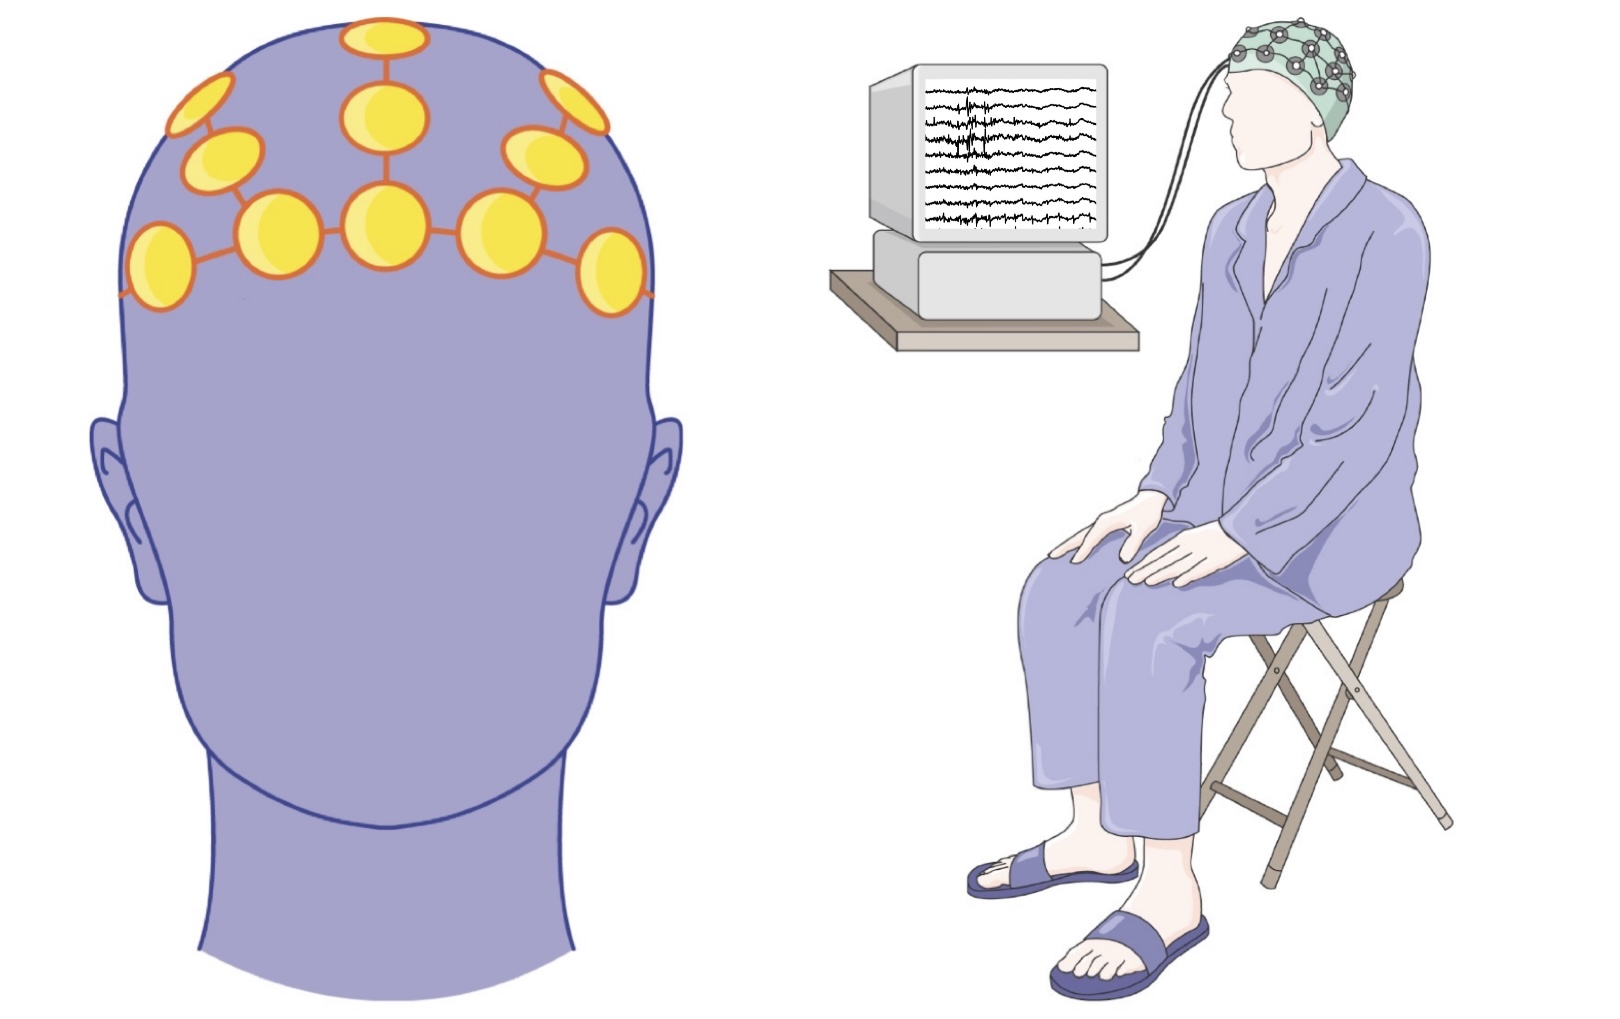
\includegraphics[width=0.6\linewidth]{figures/new_eeg_wiki.jpg}
    \caption{Illustration of the EEG method. The figures have been adapted from Wikimedia Commons with attribution to SMART-Servier Medical Art and are licensed under the Creative Commons Attribution-Share Alike 3.0 Unported license \cite{EEG_head} \cite{EEG_full_body}. The figures have been edited to remove some of the original details.}
    \label{fig:EEG}
\end{figure}


Electrical potentials generated by individual neurons are far too small to be picked up by the recording electrodes. Therefore EEG measurements primarily reflect the summation of synchronous activity from thousands of pyramidal neurons with similar spatial orientation. The activity originating from neurons with different geometric alignments cannot be picked up because their individual electrical signals tend to cancel each other out, resulting in undetectable waves at the scalp electrodes \cite{bromfield2006introduction}.

The EEG is typically described in terms of rhythmic activity and transients, which are divided into frequency bands. Frequency bands are often extracted using spectral methods, and most of the cerebral signals observed in the scalp EEG fall within the range of 1–20 Hz. Abnormal activity can broadly be classified into \emph{epileptiform} and \emph{non-epileptiform} activity. Epileptiform activity typically arises in EEG recordings of patients with epilepsy and includes spikes and sharp waves, that can be seen synchronously throughout the entire brain. In this context, spikes refer to hypersynchronized bursts from a sufficient number of neurons, arising from high-frequency bursts of action potentials \cite{bromfield2006introduction}.

Detecting and localizing abnormal electrical patterns in EEG represents an important research pursuit. One of the fundamental aspects in this field is the \emph{EEG inverse problem}, which aims to ascertain the spatial distribution of brain activity using potential measures acquired from scalp EEG recordings. Further in this chapter, we will explore the concept of the EEG inverse problem in greater detail and examine its implications for source localization.
\rednote{But first we will dive into the subject of head models for the purpose of simulating neural networks and EEG recordings.}

\rednote{Should propably come after }
\section{The Inverse Problem and Source Localization}
In the field of neuroscience, the inverse problem involves deducing the underlying neural activity responsible for a set of measured EEG data. In contrast to the \emph{forward problem}, where known parameters are used to predict the resulting EEG potential, the inverse problem lacks a unique solution. This implies that different configurations of neural sources can produce the same EEG activity distribution on the scalp \cite{hecker2021convdip}.
\rednote{Is it then possible to reach a loss equal to 0? Needs to be explained that without restictions this problem lacks uniqe solution. multipole dipoles can sup up etc... but we make restirctions and places where dipoles can be detected.}

The forward problem entails mathematically modeling of the relationship between neural current sources in the brain and the resulting EEG measurements on the scalp. This can be described as:

\begin{equation}
\Phi(t) = L \cdot p(t).
\label{eq:forward_problem}
\end{equation}

Here, $\Phi$ represents the vector of measured EEG signals at time $t$, $p(t)$ is the vector of a single cortical current dipole source at time $t$, and $L$ is the \emph{lead field matrix} that connects scalp electrode recordings with neural sources. While the full details of the lead field matrix will be explored later, for now, we envision it as a geometric arrangement linking the sensitivity of EEG measurements from diverse scalp locations to potential neural current sources within the brain.

Turning our attention to the inverse problem, its essence lies in estimating neural current sources in the brain using measured EEG data—essentially, the reverse of the forward problem. This relationship can be formulated as:

\begin{equation}
p(t) = L^{-1} \cdot \Phi(t),
\label{eq:inverse_problem}
\end{equation}

where, $L^{-1}$ denotes the inverse of the lead field matrix.

However, unlike the forward problem, the inverse problem lacks a unique solution due to its ill-posed nature. As a result, localizing the precise neural sources generating EEG signals becomes a demanding and statistically-driven endeavor. To address the complexities arising from numerous unknowns, methods such as neural networks are employed. Neural network can be designed to refine solutions to the inverse problem, providing robust and meaningful estimations of the neural sources responsible for the measured EEG data.

%In order to understand the underlaying mechanims of the brain and corresponding EEG recordings, biophysically detailed tools are essential. By accurately simulating EEG data, nonlinear optimization algorithms such as machine learning algortihms and neural networks can be utialized for solving the EEG inverse problem.

Before embarking on the utilization of artificial neural networks to solve the inverse problem, a substantial amount of appropriate EEG data is essential. This data can be obtained through simulated EEG data generated by \emph{forward modeling}. Forward modeling deals with solving the forward problem, \ref{eq:forward_problem}, and describes how the electrical activity in various regions of the human cortex gives rise to EEG signals recorded at the scalp electrodes. This process involves the use of \emph{head models} that account for the conductivity of different tissues and the geometry of the head. These head models guide the simulation process, aiding in approximating real-world EEG recordings. \rednote{head models do more than only account for the conductivity of different tissues and the geometry of the head.}


\section{Head Models}
To accurately simulate EEG data and facilitate source localization, head models that precisely represent the conductivity distribution within the human head is essential. Head models serve as computational representations of the anatomical structure of the head, encompassing the brain, skull, cerebrospinal fluid, and scalp. They play a major role in the simulation of electrical signals originating from current dipoles, their propagation through various tissue compartments, and their impact on the recorded values at scalp electrodes.

\rednote{Build up to the current dipole approximation?}
\rednote{Next, Lead Fields?}

\rednote{Is this information needed?}
EEG signals are significantly influenced by the biophysical intricacies of the head. Notably, the cerebrospinal fluid exhibits a conductivity of approximately 1.7 S/m, while the skull and scalp possess conductivities of about 0.01 S/m and 0.5 S/m, respectively. These conductivity disparities underscore the necessity for comprehensive head models that consider such variations. Beyond conductivity, these models also account for the influence of tissue arrangement on EEG signals, such as whether a neuronal population resides within a \emph{sulcus} or a \emph{gyrus} \cite{naess2021biophysically}. By employing such a biophysically detailed head model, one can more accurately simulate the impact of various tissues on the distribution of extracellular potential. As a result, this model offers a heightened level of precision in representing EEG signals, leading to improved accuracy in EEG source localization solutions.


\subsection{The New York Head Model}
The New York Head model (NYHM), developed by the Biomedical Engineering Department at the City University of New York, is a highly detailed computer model tailored for simulating electrical brain activity, with an emphasis on EEG source localization. Grounded in high-resolution anatomical MRI data from 152 adult heads, this model allows the segmentation of six distinct tissue types within the head: scalp, skull, cerebrospinal fluid, gray matter, white matter, and air cavities. Its high level of detail and accuracy makes it an excellent tool for simulating and comprehending brain activity in a realistic manner. Presenting a three-dimensional representation of the head and brain, coupled with precise information about tissue geometry and electrical properties, this head model will be utilized in our work within the context of EEG simulation to generate the data used for dipole source localization.

To precisely calculate EEG signals recorded at various scalp locations, the New York Head Model (NYHM) relies on a fundamental principle known as the \emph{reciprocity theorem}. This theorem states that if you swap the positions of a dipole source and a measurement point, the measured value for the potential will remain the same. We calculate what is called the \emph{lead field} by simulating a current dipole source at an electrode location and computing the resulting potential distribution at different points within the cortex. The lead field values are thus the EEG signals that would be measured at the electrode location when a source is positioned at one of the points in the cortex \cite{naess2021biophysically}. This turns out to be more efficient than simulating the EEG signals that would be measured at the electrode positions from the electrical signature of a single dipole within the cortex. The efficiency of this approach becomes evident due to the reduced computational demands when simulating EEG signals measured at recording electrodes. Specifically, simulating the propagation of the electrical field from a single dipole location, propagating through the densely distributed cortex and reaching the recording electrodes, requires tens of thousands of calculations, corresponding to the vast number of dipole locations within the cortex. In contrast, simulating the electrical field from the recording electrodes through the cortex requires calculations equal to the number of recording electrodes, which is significantly smaller, thus greatly simplifying the computational load.


%The reason for this is simply because simulating the EEG signals measured at a set of recording electrodes, requires less computations than simulating the EEG signals for a much larger number of dipole locations, with a higher density.
\rednote{This flipped approach is more efficient?}
\rednote{Potential vs. electric field.}

To construct the NYHM's lead field matrix (\(L\)), the researchers behind the model have performed these calculations for 231 electrode positions on the scalp and 70,000 possible dipole source locations within the cortex. Each location point includes the $x$-, $y$-, and $z$-coordinates, with the $x$-coordinate ranging from -72 to 72 mm, the $y$-coordinate spanning -106 to 73 mm, and the $z$-coordinate extending from -53 to 82 mm. This lead field matrix establishes the mathematical relationship between a current dipole moment within the brain cortex and the resulting EEG signals.
Each row of the matrix corresponds to the
Mathematically, the lead field matrix is defined as:
\begin{equation}
  L_{ij} = \frac{E_j^{(i)}}{I}, \quad \text{for } j = x, y, z.
  \label{eq:LeadFieldMatrix}
\end{equation}
Here, $I$ represents the injected current at the electrode locations, and $\mathbf{E}^{(i)} = (E_x^{(i)}, E_y^{(i)}, E_z^{(i)})$ is the resulting electric field in the brain at . The row index $i$ spans from 1 to $231 \cdot 70,000$. This use of the reciprocity principle greatly simplifies computations because it means that solutions to the forward problem are precomputed for every current dipole location. Consequently, the EEG signal $\Phi$, which encapsulates the values measured at each of the recording electrodes resulting from a current dipole, can be calculated through a straightforward matrix multiplication:
\begin{equation}
  \Phi = (\phi_0, \dots, \phi_{70,000})
  \Phi = L \mathbf{p},
  \label{eq:EEG_signal_matrix}
\end{equation}
where the current dipole moment $\mathbf{p} = (p_x, p_y, p_z)$ holds the dipole's magnitude in the \(x, y, z\)-directions respectively.

For further comprehensive details about the New York Head model, we refer readers to Huang, Parra, and Haufe (2016) \cite{huang2016new}.


\section{The Current Dipole Approximation}

By accurately simulating EEG data, nonlinear optimization algorithms such as neural networks can be utilized for solving the EEG inverse problem. However, the simulation of intricate neuronal dynamics is a computationally expensive and complex task. \rednote{Not correct. Head models are always based on dipole approximation, and so are lead field matrices.} An approximation that address this challange and simplifies the simulation phase is the \emph{current dipole approximation}. This approximation is rooted in the observation that the neuron's contribution to the extracellular potential $V_e$ becomes increasingly more dipole-like with an increasing distance.

The key insight behind the current dipole approximation lies in the \emph{multipole expansion}, a technique that comes to our aid when the recording point is situated at a significant distance from the source distribution. While electrical charges within neural tissue can give rise to the formation of current multipoles, the multipole expansion theorem offers a method to express the extracellular potential, denoted as $V_e(R)$, in terms of various pole contributions. In the context of EEG signals, employing this theorem reveals that $V_e(R)$ can be effectively approximated by a single dipole \cite{brainmodel2022}. \rednote{Wikipedia has also been used here. Check with book that everything is correct.}

Neuronal multipoles depend on the spatial arrangement and symmetry of the charge distribution and result from the interplay of current sources and sinks \cite{wiki:multipoles}. The expression for the extracellular potential associated with different multipole orders may take complicated forms, and be hard to interpreted. However, when the distance $R$ from the center of the source to the recording point surpasses the extent of the source, the applicability of multipole expansion becomes evident \cite{jackson1999classical} \rednote{is this correct?}. This expansion are often beneficial as usually only the first few terms are needed in order to provide an accurate approximation of the original funtion, as we will se now. Using the multipole expansion theorem, the representation of the extracellular potential $\phi(R)$ takes the form:

\begin{equation}
  V(R) = \frac{C_{\text{monopole}}}{R} + \frac{C_{\text{dipole}}}{R^2} + \frac{C_{\text{quadrupole}}}{R^3} + \frac{C_{\text{octopole}}}{R^4} + ... .
\label{eq:extracellular_potential}
\end{equation}

where the numerators represents the contributions to the extracellular potential. The terms denoted $C_\text{monopole}$, $C_\text{dipole}$ and $C_\text{quadrupole}$ represents contributions to the extracellulat potential, $V_e$, and can in general be extremely complicated as they depend on the relationship between radial coordinates and symmetry of the current source and measurement electrode. We note that the contributions beyond the dipole term decay more rapidly with distance $R$. This means that in scenarios where we are considerably distant from the source distribution, the higher-order terms become negligible, leaving us primarily with the monopole and dipole contribution. This brings us to another interesting observation: The monopole contribution vanishes, stemming from the fact that the net sum of currents over a neuronal membrane is invariably zero. Consequently, we are left with an approximation of the extracellular potential, $V_e$, that relies solely on the dipole contribution:

\begin{equation}
V_e(\textbf{r}) \approx \frac{C_{\text{dipole}}}{R^2} = \frac{1}{4\pi\sigma}\frac{|\textbf{p}| \text{cos} \theta}{\lvert\textbf{r}-\textbf{r}_p\rvert^2}.
\label{eq:extracellular_potential_approximation}
\end{equation}

Here we have substituded for $C_\text{dipole}$ in terms of other properties. Here $p$ symbolizes the current dipole moment within a medium of conductivity $\sigma$. The distance between the current dipole moment at $\textbf{r}_p$ and the electrode location $\textbf{r}$ is denoted as $R = |\textbf{R}| = |\textbf{r} - \textbf{r}_p|$. Additionally, $\theta$ signifies the angle between $\textbf{p}$ and $\textbf{R}$. This equation is recognized as the dipole approximation and stands as a reliable method for calculating the extracellular potential, particularly when the distance $R$ significantly surpasses the dipole length. This condition is inevitably met in EEG studies, as the dipole length cannot exceed the depth of the cortex, while EEG electrodes are typically positioned several centimeters away from the cortical surface on the scalp \cite{naess2021biophysically}.

Consequently, we have connected the concept of multipole expansion with the validity of the dipole approximation. Through multipole expansion, we can comprehend the intricate extracellular potential in terms of various contributions, and by carefully considering their behavior, we arrive at the precise dipole approximation.

In Figure \ref{fig:dipole_pattern}, we have provided a simulation of the extracellular potential generated by a neuron in response to a single synaptic input, where the spatial distribution of membrane current was explicitly taken into consideration. The Figure has been collected from work done by Torbjørn Ness and Gaute Einevoll. This simulation aligns with the dipole approximation, as it clearly visualizes the distribution of electric charge in the extracellular potential of the neuron's surroundings, revealing distinct dipole patterns when observed from a greater distance.

\begin{figure}
    \centering
    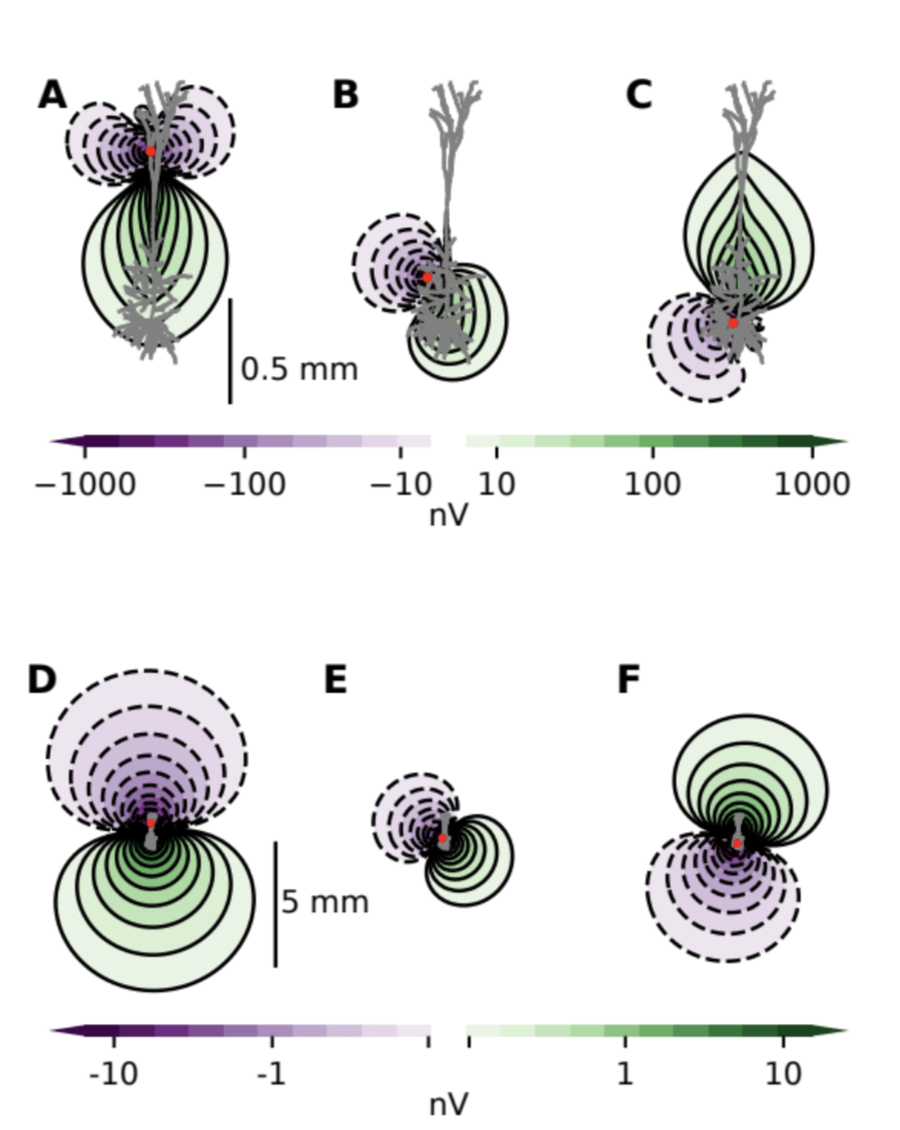
\includegraphics[width=\linewidth]{figures/dipole_pattern.png}
    \caption{Simulation of extracellulat potential showing distinct dipole pattern. The figure has been provided from my supervisiors Torbjørn Ness and Gaute Einevoll.}
    \label{fig:dipole_pattern}
\end{figure}

\section{The Effect of Dipole Orientation}
Figure \ref{fig:gyrus_and_sulcus_EEG} and \ref{fig:dipole_orientation} are borrowed from work done by Tornjørn Ness and Gaute Einevoll, and illustrate the impact of dipole orientation on EEG outcomes. Figure \ref{fig:gyrus_and_sulcus_EEG} represent the EEG signals obtained from two manually selected dipole locations within the New York head model. These dipoles are situated in a gyrus and a sulcus, respectively, and exhibit distinct EEG patterns. In general, the contribution of an individual current dipole to the EEG signal is maximized when the dipole is perpendicularly situated within a gyrus, as depicted in Figure \ref{fig:gyrus_and_sulcus_EEG}B. Contrastingly, when a dipole is placed in a sulcus with a perpendicular orientation, a significant EEG contribution may still be observed, however unlike the dipole in the gyrus, it exhibits a more dipolar pattern, as shown in Figure \ref{fig:gyrus_and_sulcus_EEG}C.


\begin{figure}[!htb]
    \centering
    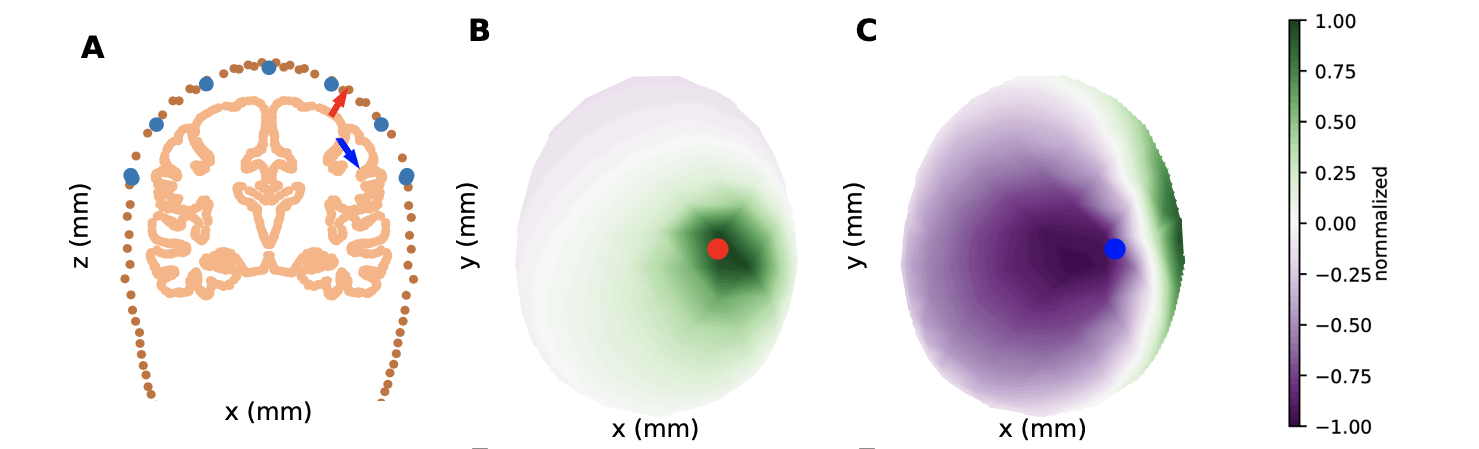
\includegraphics[width=\linewidth]{figures/gyrus_and_sulcus_EEG.png}
    \caption{A: Two selected dipole locations in the New York head model: one in a gyrus (red) and one in a sulcus (blue). The head model is viewed from the side (x, z-plane). Close to the chosen cross-section plane, EEG electrode locations are marked in light blue. Available dipole locations near the cortical cross-section form an outline of the cortical sheet and are marked in pink. The current dipole moment for all cases was 1 nAm. B: Interpolated color plot of EEG signal from the gyrus dipole, viewed from the top (x, y-plane). The plotted EEG signal is scaled, with a maximum value of 1.1 $\mu$V. C: Interpolated color plot of EEG signal from the sulcus dipole. The plotted EEG signal is scaled, with a maximum value of 0.7 $\mu$V. This Figure is borrowed from work done by Torbjørn Ness and Gaute Einevoll \cite{naess2021biophysically}.}
    \label{fig:gyrus_and_sulcus_EEG}
\end{figure}

Further, Figure \ref{fig:dipole_orientation} depicts the EEG signals from identical dipoles positioned in various folding patterns of the cortical surface. These patterns align with the previous observations, as they showcases that the orientation of the current dipole moment significantly influences the EEG outcome. Firstly, Figure \ref{fig:dipole_orientation}A and \ref{fig:dipole_orientation}C provide an expanded illustration of the aforementioned scenarios, incorporating additional dipole moments located in a gyrus and a sulcus, respectively. In Figure \ref{fig:dipole_orientation}B, where a collection of dipoles points randomly upwards and downwards, the EEG signal contribution appears to diminish significantly. Conversely, when the dipoles align in the depth direction of the cortex and are distributed across both gyrus and sulcus, we can expect an EEG contribution in between what we saw from Figure \ref{fig:dipole_orientation}A and \ref{fig:dipole_orientation}B, as depicted in Figure \ref{fig:dipole_orientation}D. Lastly, Figure \ref{fig:dipole_orientation}E demonstrates the minimal EEG contribution observed when the dipoles are divided between two opposing sulci.


\begin{figure}[!htb]
    \centering
    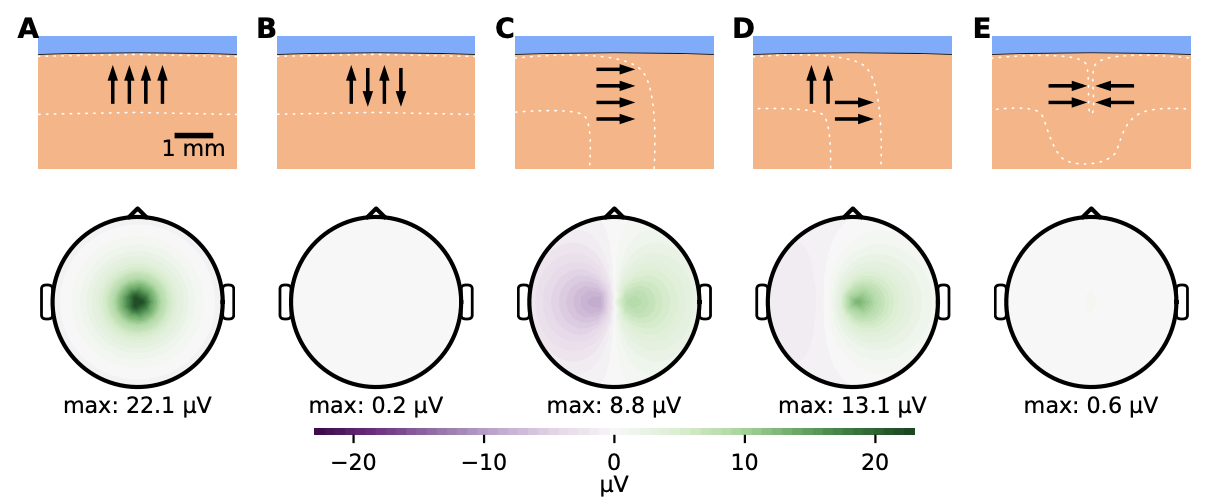
\includegraphics[width=\linewidth]{figures/dipole_orientation.png}
    \caption{Different folding patterns of the cortical surface are represented by white dashed lines. EEG signals are calculated from four identical current dipoles with varying orientations. A: Dipoles aligned in the same direction within a gyrus. B: Dipoles pointing in opposite directions within a gyrus. C: Dipoles aligned in the same direction within a sulcus. D: Dipoles distributed between a gyrus and a sulcus, pointing towards the cortical surface. E: Dipoles divided between opposing sulci, pointing towards the cortical surface.
    Each panel features a dipole moment magnitude of 10 nAm, and the dipoles are positioned at the centers of the arrows in the top row. This Figure is borrowed from work done by Torbjørn Ness and Gaute Einevoll \cite{naess2021biophysically}.}
    \label{fig:dipole_orientation}
\end{figure}

% This is not the case for a simple dipole moment, but might be an issue when giving the populations a radii
% In our analysis, we simplify the scenario by considering one current dipole at a time, which allows us to avoid cancellations of potentials and obtain simpler EEG potentials. While this simplification may not capture the full complexity of neural activity, it provides us with a clearer understanding of the relationship between dipole orientation and EEG signals.



\section{Solving the EEG inverse problem}
In this chapter, we have explored the fundamental concepts that underpin the investigation of the inverse problem in EEG source localization. With this groundwork in place, we now turn our attention to the subsequent chapters, where we transition from theory to application.

In the next chapter, we delve into practical implementation by simulating EEG data. Utilizing the New York Head Model and current dipole approximation, we create synthetic EEG data that closely resembles real-world scenarios. This simulated data, generated using the principles discussed in this chapter, serves as a crucial foundation for the subsequent chapters. It brings us a step closer to addressing the EEG source localization challenge.

Chapter 4 explores the methods of machine learning and neural networks. Building upon the simulated EEG data, we construct a sophisticated neural network designed to address the inverse problem efficiently. By the use of computational techniques, our aim is to bridge the gap between theoretical understanding and real-world applications.

\end{document}
